\documentclass[review]{elsarticle}

\usepackage{lineno,hyperref}

\usepackage{amsmath}
\usepackage{amsfonts}
\usepackage{amsthm}
\usepackage{url}
\DeclareMathOperator*{\argmin}{argmin}
\newcommand*{\argminl}{\argmin\limits}
\newtheorem{prop}{Proposition}

\modulolinenumbers[5]

\journal{Statistics and Probability Letters}

%%%%%%%%%%%%%%%%%%%%%%%
%% Elsevier bibliography styles
%%%%%%%%%%%%%%%%%%%%%%%
%% To change the style, put a % in front of the second line of the current style and
%% remove the % from the second line of the style you would like to use.
%%%%%%%%%%%%%%%%%%%%%%%

%% Numbered
%\bibliographystyle{model1-num-names}

%% Numbered without titles
%\bibliographystyle{model1a-num-names}

%% Harvard
%\bibliographystyle{model2-names.bst}\biboptions{authoryear}

%% Vancouver numbered
%\usepackage{numcompress}\bibliographystyle{model3-num-names}

%% Vancouver name/year
%\usepackage{numcompress}\bibliographystyle{model4-names}\biboptions{authoryear}

%% APA style
%\bibliographystyle{model5-names}\biboptions{authoryear}

%% AMA style
%\usepackage{numcompress}\bibliographystyle{model6-num-names}

%% `Elsevier LaTeX' style
\bibliographystyle{elsarticle-num}
%%%%%%%%%%%%%%%%%%%%%%%

\begin{document}

\begin{frontmatter}

\title{A Stopped Negative Binomial Distribution}
\tnotetext[mytitlenote]{This research was supported by grants R01CA131301, 
R01CA157749, R01CA148996, R01CA168733, and PC50CA196530 awarded by the 
National Cancer Institute, and support from the Yale Comprehensive Cancer 
Center.}

%% Group authors per affiliation:
%\author{Elsevier\fnref{myfootnote}}
%\address{Radarweg 29, Amsterdam}
%\fntext[myfootnote]{Since 1880.}

%% or include affiliations in footnotes:
\author[mymainaddress]{Michelle DeVeaux}
\ead{michelle.deveaux@yale.edu}

\author[mymainaddress]{Michael J. Kane\corref{mycorrespondingauthor}}
\cortext[mycorrespondingauthor]{Corresponding author}
\ead{michael.kane@yale.edu}

\author[mymainaddress]{Daniel Zelterman}
\ead{daniel.zelterman@yale.edu}

\address[mymainaddress]{Department of Biostatistics\\ School of Epidemiology and Public Health\\ Yale University, New Haven, CT}

\begin{abstract}
This paper introduces a novel discrete distribution suggested by curtailed
sampling rules common in early-stage clinical trials. We derive the
distribution of the smallest number of independent and identically
distributed Bernoulli trials needed in order to observe either $s$ successes 
or $t$ failures. The closed-form expression for the distribution as well as 
its characteristics and properties are explored.
\end{abstract}

\begin{keyword}
discrete distribution\sep curtailed sampling
\end{keyword}

\end{frontmatter}

\linenumbers

\section{Introdution and Motivation}

Consider a prototypical Phase II single-arm clinical trial. 12 patients
are enrolled and treated. If at least 2 of those patients respond
favorably, then the trial will proceed to the next stage. If fewer than 
two respond then the trial would have been terminated.

The maximum sample size is 12 but the number of patients necessary to
reach any endpoint could be less. Our goal is to describe the distribution of
the enrollment size. This distribution will be used for planning purposes. 
If all 12 patients are enrolled at once, as in the classic
design, then the sample size is 12. However, in most clinical trials, the
patients are enrolled sequentially, often with one patient's outcome realized
before the next one enters the trial. In the present example, observing two
successful patients allows us reach one endpoint so the sample required
could be as small as two - 12 might not be necessary. Similarly 11
observed treatment failures also ends the stage. This sampling mechanism, in
which the experiment ends as soon as any of the endpoints is reached, is
call {\em curtailed sampling}. Under curtailed sampling the range of the
sample size is between two and 12.

Assume each of patient outcome can be modeled as an independent,
identically distributed Bernoulli($p$) random variable. The trial is realized
as a sequence of these random variables that stops when either a
specified number of success or failures is reached. In the
previous example suppose two successes were reached after enrolling 10
patients (one in the third step and one at the $10^{th}$). The sample
path is illustrated
in Fig.~\ref{fig:kane_viz}. The vertical axis denotes the number of
successful outcomes. The horizontal axis counts the number of patients that
have been enrolled. The horizontal and vertical boundaries represent
endpoints for the trial.

\begin{figure}[t!]
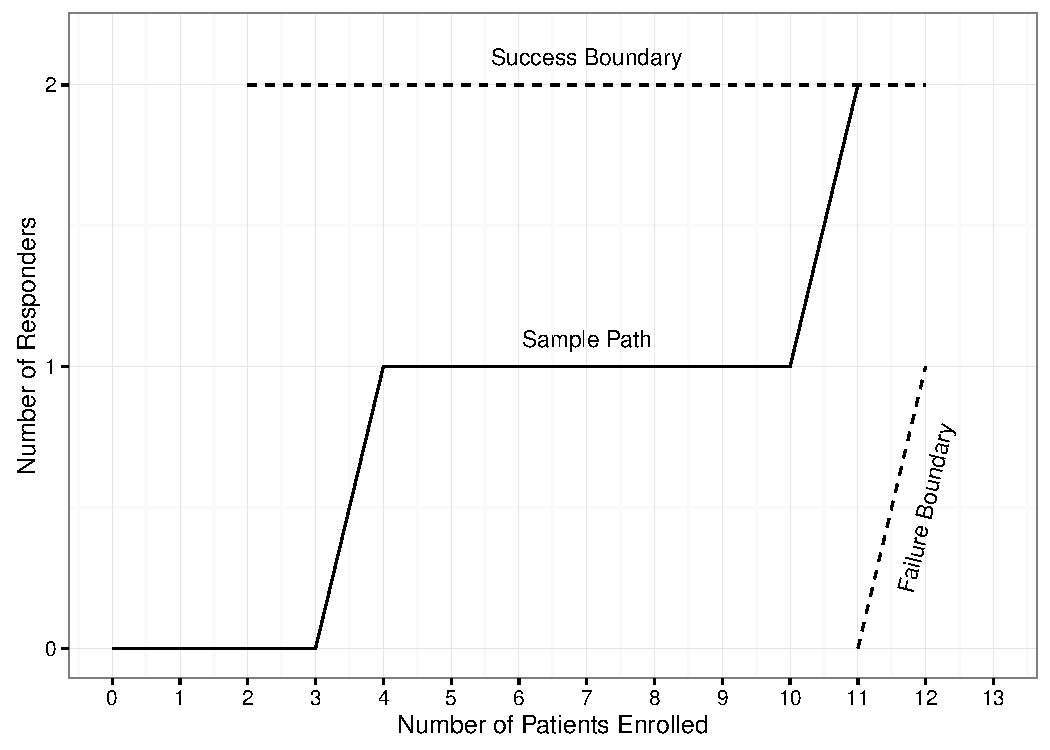
\includegraphics[width=\textwidth]{KanePlot.pdf}
\caption{
A hypothetical realization of a trial.
}
\label{fig:kane_viz}
\end{figure}

The rest of this paper derives the distribution for the number of
patients needed to end a trial and explores the characteristics and
properties of this distribution.
The next section introduces our notation and basic results
including the density of the distribution along with a description of
it's relation to other distributions. Sections 2 derives the distribution
based on a defined Bernoulli process and give some basic properties.
Section 3 provides a connection to the Binomail tail probability.
Section 4 derives the posterior distribution using a Beta prior.
Section 5 provides a brief discussion on the use of the distribution
in clinical trials along with future avenues for generalization.

\section{Distributional Result}
\label{notation.section}

Let $\,b_1, b_2, \ldots \,$ denote a sequence of independent, identically
distributed, Bernoulli random variables with $\mathbb{P}[b_i=1]=p$ and
$\mathbb{P}[b_i = 0] = 1-p$, for
probability parameter $0\leq p \leq 1$. In the clinical trial setting
$\,b_i = 1$ corresponds to a successful outcome.  Let $s$ and $t$ be
positive integers.  Define the stopped negative binomial (SNB) random
variable $Y$ as the smallest
integer value such that $\,\{b_1, \ldots , b_Y\}\,$ contains {\em either}
$\,s\,$ successes {\em or} $\,t\,$ failures. That is, either
$\sum_i^Y b_i = s$ or $\sum_i^Y 1-b_i = t$.

The distribution of $\,Y\,$ has support on integer values in the range
\begin{equation*}               
     \min(s,t) \leq \; Y \;\leq s+t-1  \label{range.y.eq}
\end{equation*}
and it is distributed as
\begin{equation} \label{eqn:pmf}
\mathbb{E}\  I_{\{Y=k\}} = S(k, p, s) \ I_{\{s \leq k\}} + 
  S(k, 1-p, t) \ I_{\{ t \leq k \}}
\end{equation}
where $I_{\{f\}}$ is one if $f$ is true and zero otherwise and
\begin{equation} \label{eqn:N}
S(k, p, s) = {k-1 \choose s-1} p^s (1-p)^{k-s} 
\end{equation}
$S$ is the negative binomial probability

To prove the result in Eqn.~\ref{eqn:pmf} consider the
process $\mathbf{X} = \left\{X(k) : k = 0,1,... \right\}$
with $X(0)=0$ and
\begin{equation*} \label{eqn:proc}
X_{k+1} = X_k + b_{k+1} \ I_{\{ k-t < X_k < s\}}.
\end{equation*}
The process can be conceptualized as a series of coin
flips that stops when either $s$ successes or $t$ failures are reached.
At each step a coin is flipped. If it is heads, the process advances
one diagonally in the
positive horizontal and vertical direction.
Otherwise, it advances in the positive horizontal direction only. The
process stops when either $X_k = s$ or $X_k = k-t$.

\begin{prop}
The distribution of the stopping time
$\argminl_k \left\{ X_k \geq s \cup X_k \leq k-t \right\}$
is equal to Eqn.~\ref{eqn:pmf}.
\end{prop}
\begin{proof}
%The proof will proceed in two parts. First, a combinatorial justification 
%will be given for the probability mass value on each element of the support. 
%Second, it will be shown that the sum of the masses over the support sums to 
%one.

The probability a given realization of $\mathbf{X}$ reaches $s$ at
the $k$th outcome is the probability that, at time $k-1$ there are $s-1$
successful outcomes and $k-s$ unsuccessful outcomes multiplied by
the probability of a
success at time $k$. 
\begin{equation} \label{stop_s}
S(k, p, s) = {k-1 \choose s-1} p^s (1-p)^{k-s}
\end{equation}
The probability a given realization reaches $k-t$
is the probability that, at outcome $k-1$ there are $k-t$ successful outcomes
and $t-1$ unsuccessful outcomes multiplied by the probability of an
unsuccessful outcome at time $k$.  
\begin{equation} \label{stop_t}
S'(k, p, t) = {k-1 \choose k-t} p^{k-t} (1-p)^t
\end{equation}
It can be shown that $S(k, p, s) = S'(k, 1-p, s)$ by realizing that 
${k-1 \choose k-s} = {k-1 \choose s-1}$.

To show that sum of Eqn. \ref{stop_s} and \ref{stop_t} sum to one
over their support 
\begin{align} \label{eqn:sum_proof}
R &= \sum_{k=s}^{s+t-1} S(k, p, s) + \sum_{k=t}^{s+t-1} S(k, 1-p, t) \\
  &= \sum_{k=s}^{s+t-1} {k-1 \choose s-1} p^s (1-p)^{k-s} + \sum_{k=t}^{s+t-1} {k-1 \choose k-t} p^{k-t} (1-p)^t
\end{align}
substitute $i=k-s$ in the first summation and $j=k-t$ in the second.
Then $R$ can be written
as the cumulative distribution function of two
negative binomial distributions
\begin{equation} \label{eqn:transformed_sum}
R = \sum_{i=0}^{t-1} {i+s-1 \choose i} p^s (1-p)^i \; + \;
\sum_{j=0}^{s-1} {j+t-1 \choose j} p^j (1-p)^t.
\end{equation}

Let $\mathcal{I}_p(s, t)$ be the {\em regularized incomplete beta function}
and recall this function satisfies 
$\mathcal{I}_p(s, t) = 1-\mathcal{I}_{1-p}(t, s)$ \citep{Abramowitz1964}.
\begin{align*}
R = \sum_{i=0}^{t-1} &{i+s-1 \choose i} p^s (1-p)^i +
\sum_{j=0}^{s-1}  {j+t-1 \choose j} p^j  (1-p)^t \\
   &= 1-\mathcal{I}_p(s, t) + 1 - \mathcal{I}_{1-p}(t, s) \\
   &= 1. 
\end{align*}
\end{proof}

\section{Shape and Basic Properties}

\begin{figure}[p!]
\begin{center}
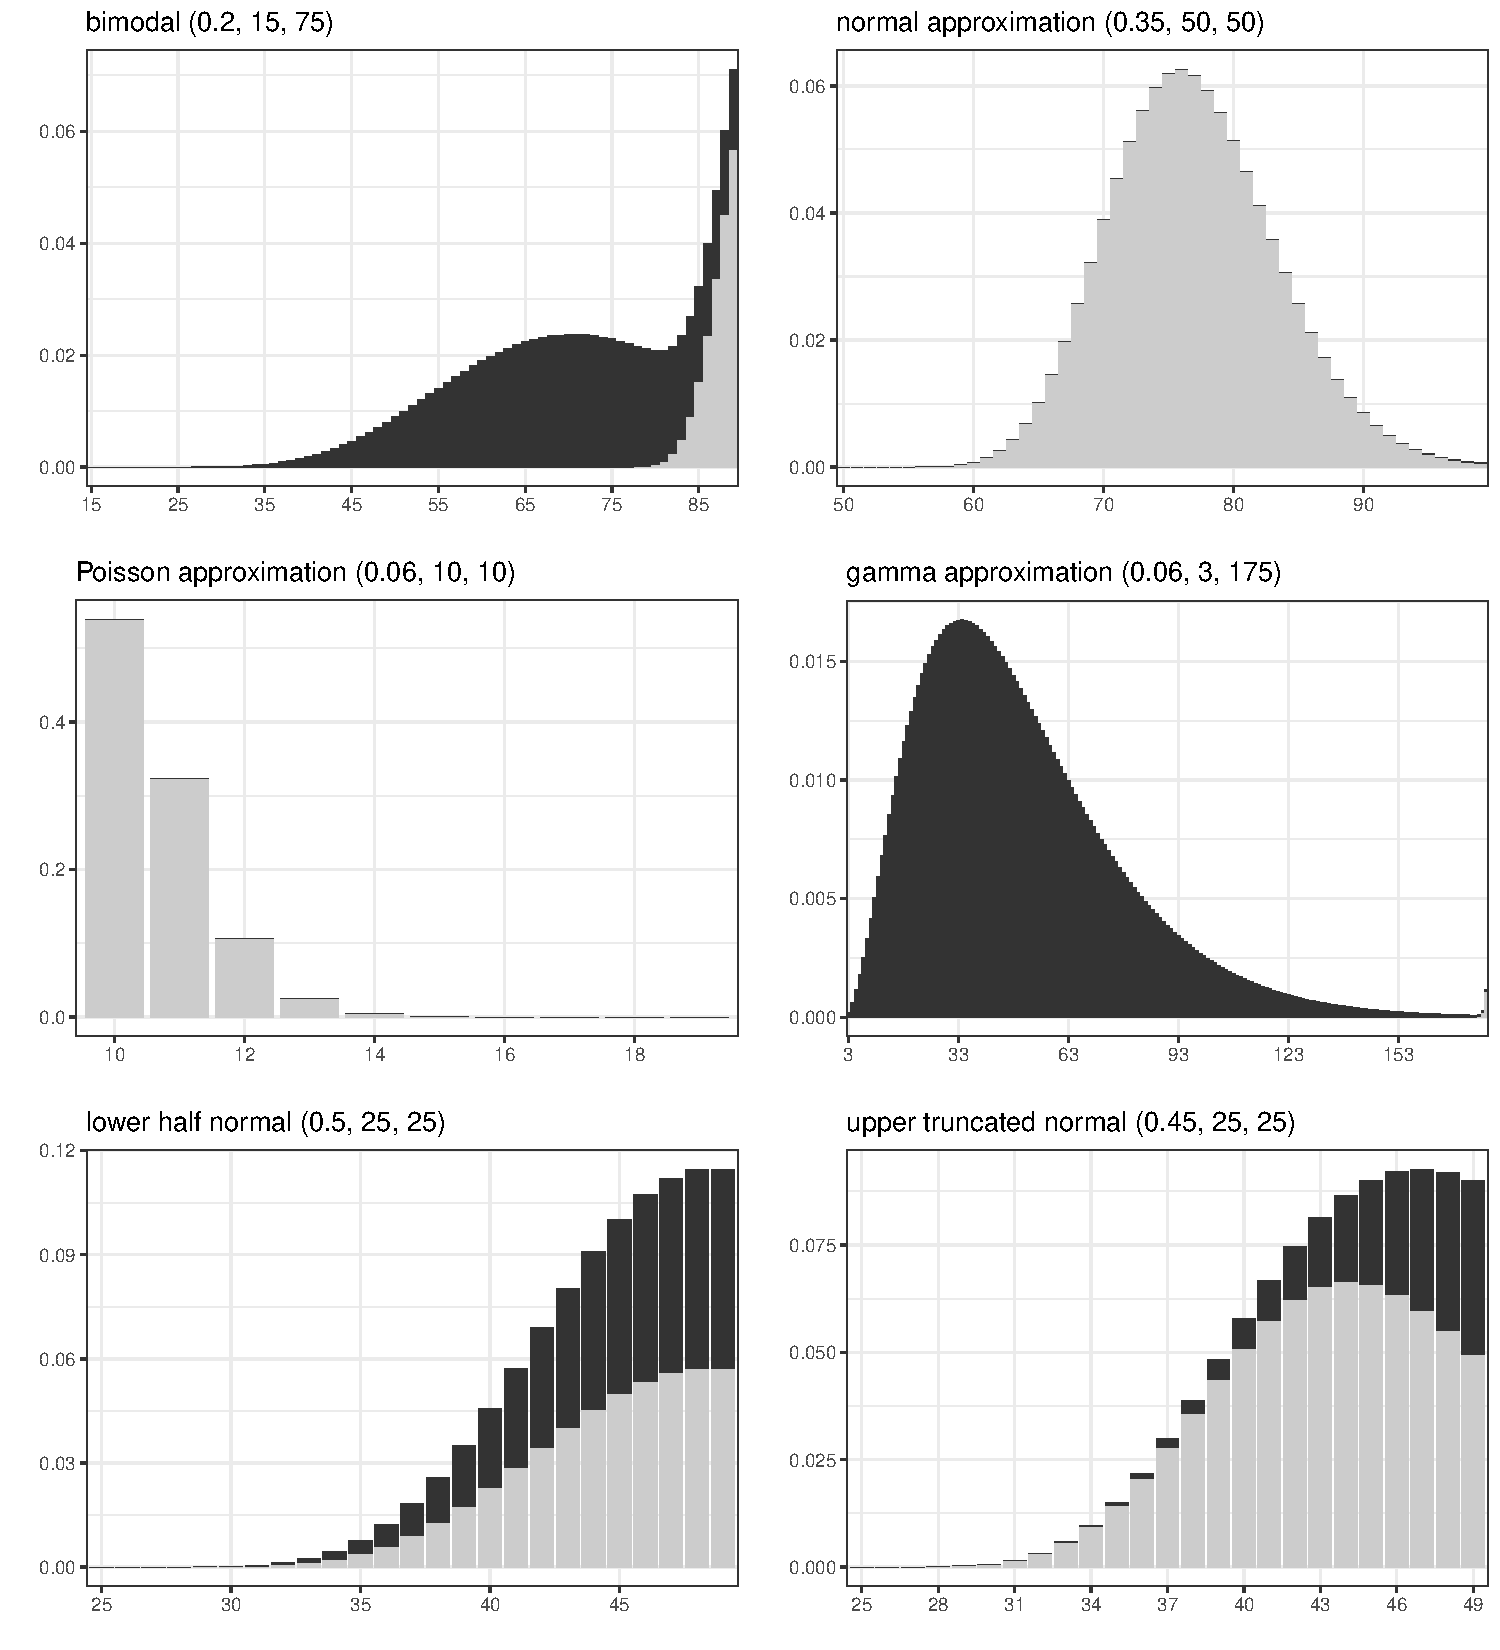
\includegraphics[width=\textwidth]{shapes.pdf}
\end{center}
\caption{Different shapes of the SNB distribution with parameters ($s$, $t$, $p$), as given. Red indicates mass contributed by hitting $s$, teal indicates
mass contributed by hitting $t$. \label{shapes.fig}}
\end{figure}

The probability mass function of $\,Y\,$ has a variety of shapes for different 
choices of the parameters $(s,\, t,\,p)$.  These shapes are illustrated in 
Fig.~\ref{shapes.fig}. The SNB is related to the negative binomial 
distribution. Specifically, if $t$ is large then the $Y-s$ has a negative 
binomial distribution with
\begin{equation*}                                    %   (1)   
\mathbb{P}[Y=s+j]        \label{nb1.eq}          
  = {{s+j-1}\choose{s-1}} p^s (1-p)^j
\end{equation*}
for $\,j=0, 1,\ldots\,$. A similar statement can be made when $s$ is large
and $t$ is small.

For the special case of $\,s=t,$ the distribution of $\,Y\,$ is the
riff-shuffle, or minimum negative binomial distribution~\citep{Uppuluri1970}.
Similar derivations of the closely-related maximum negative binomial 
discrete distributions also appear in~\cite{Zhang2000}
and \cite{Zelterman2005}.
The maximum negative binomial is the smallest number of outcomes necessary to 
observe at least $c$ successes {\em and} $c$ failures, but the SNB givethe 
number of coin flips to observe {\em either} $s$ heads or $t$ tails.

\section{Connection to the Binomial Tail Probability}


\begin{prop} Let $Y$ be distributed as SNB($p$, $s$, $t$) and let 
$B$ be distributed Binomial with size $n=s+t-1$ and success probability
$p$. Then
\begin{equation}
\mathbb{P}[B \geq s] = \mathbb{P} [Y \leq n | \text{\#success} = s].
\end{equation}
That is, the probability that the number of successes is at least $s$
in the Binomial model is the same that the trial stops with $s$ 
successes in the SNB model.
\end{prop}
\begin{proof}
The Binomial tail probability is
\begin{align*}
\mathbb{P}[B \geq s] &= \sum_{k=s}^{s+t-1} {n \choose k} p^k (1-p)^{n-k} \\
  &= 1 - \sum_{k=0}^{s-1} p^k (1-p)^{n-k} \\
  & 1 - \mathcal{I}_{1-p}.
\end{align*}
Next, consider the SNB probability
\begin{equation*}
\mathbb{P} [Y \leq n | \text{\#success} = s] = \sum_{k=s}^{s+t-1}
  {k-1 \choose s-1} p^s (1-p)^k-s.
\end{equation*}
Let $i=k-s$ then using the fact that ${i+s-1 \choose s-1} = {i+s-1 \choose i}$
the summation can be rewritten as
\begin{align}
\mathbb{P} [Y \leq n | \text{\#success} = s] &= \sum_{i=0}^{t-1} 
  {i+s-1 \choose i} p^s (1-p)^i\\
  &= 1 - \mathcal{I}_{1-p}(t, s).
\end{align}
\end{proof}

\section{The Moment Generating Function}

\begin{prop} Let $S$ be distributed SNB with parameters $p$, $s$, and $t$.
Then the moment generating function (MGF) of $S$ is
\begin{equation} \label{eqn:mgf}
\mathbb{E}~e^{xS} = \frac{p e^x}{1 - qe^x} \mathcal{I}_{qe^x} (s, t) + 
  \frac{qe^x}{1-pe^x} \mathcal{I}_{pe^x}(s, t)
\end{equation}
for $q = 1-p$ when $x \leq -\log(q)$ and $x \leq -\log(p)$.
\end{prop}
\begin{proof}
By definition, the MGF of the SNB is:
\begin{equation*}
\mathbb{E}~e^{xS} = \sum_{k=s}^{s+t-1} {k-1 \choose s-1} p^s q^{k-s} e^{kx} 
  + \sum_{k=t}^{s+t-1} {k-1 \choose k-t} p^{k-t} q^t e^{kx}
\end{equation*}
and can be rewritten as:
\begin{equation} \label{eqn:first_sum}
\mathbb{E}~e^{xS} = \sum_{k=s}^{s+t-1}{k-1 \choose s-1} (pe)^{sx} (qe^x)^{k-s} 
  + \sum_{k=t}^{s+t-1}{k-1 \choose k-t} (qe^x)^t (pe^x)^{k-t}.
\end{equation}
Taking the first summation in Equation \ref{eqn:first_sum}:
\begin{align*}
\sum_{k=s}^{s+t-1}{k-1 \choose s-1} (pe)^{sx} (qe^x)^{k-s} &= 
  \left(\frac{pe^x}{1 - qe^x}\right)^s \ \ \sum_{k=s}^{s+t-1} {k-1 \choose s-1} 
    (qe^x)^{k-s} (1-qe^x)^s) \\
  &= \left(\frac{pe^x}{1 - qe^x}\right)^s \mathcal{I}_{qe^x}(s, t).
\end{align*}
Since the incomplete beta function has support on zero to one
$qe^x \leq 1$. This implies that $x \leq -\log(q)$.

A similar expression can be derived using the same calculation with
the constraint that $x \leq -\log(p)$. The result
follows from the afore mentioned property of the regularized incomplete
beta function.
\end{proof}

\section{The Posterior Distribution}

Let us assume that $p$ has a Beta distribution, with constant prior
parameters $\alpha$ and $\beta$. Then the closed form
posterior distribution of the SNB is
\begin{align}
f \left(k | \mathbf{b}, \alpha, \beta \right) &= 
  {k-1 \choose s-1} \frac{B\left(\alpha+s, k-s+\beta \right)}{B(\alpha, \beta)} 
  \ I_{\{s \leq k \leq s+k-1\}} + \nonumber \\
  & {k-1 \choose k-t} 
  \frac{B\left(\alpha + k - t, t+\beta\right)}{B(\alpha, \beta)} 
  \ I_{\{t \leq k \leq s+k-1\}}
\end{align}
where $B$ is the Beta function and $\mathbf{b}$ is the realization
of Bernoulli data.

\begin{prop}
The posterior PMF of the Stopped Negative Binomial distribution with a Beta($\alpha$, $\beta$) prior is:
\begin{align} \label{eqn:posterior}
f(k | s, t, \alpha, \beta) &= 
  {k-1 \choose s-1} \frac{B\left(\alpha+s, k-s+\beta \right)}{B(\alpha, \beta)} 
    \ I_{\{s \leq k \leq s+k-1\}} \ + \nonumber \\
  & {k-1 \choose k-t} 
    \frac{B\left(\alpha + k - t, t+\beta\right)}{B(\alpha, \beta)} 
    \ I_{\{t \leq k \leq s+k-1\}}
\end{align}
where $B$ is the Beta function.
\end{prop}
\begin{proof}
For notational simplicity, assume that $s,t \leq k \leq s+t-1$. When this is not the case appropriate terms should be removed as dictated by the indicator functions.
\begin{align*}
f(k | s, t, \alpha, \beta) = \frac{1}{B(\alpha, \beta)} & \int_0^1 {k-1 \choose s-1} p^{\alpha +s -1} \left(1-p\right)^{k-s+\beta-1} + \\
 & {k-1 \choose k-t} p^{k-t+\alpha-1}\left(1-p\right)^{t+b-1} dp \\
= \frac{1}{B(\alpha, \beta)}  {k-1 \choose s-1} & \int_0^1  p^{\alpha +s -1} \left(1-p\right)^{k-s+\beta-1} dp + \\
 & \frac{1}{B(\alpha, \beta)} {k-1 \choose k-t} \int_0^1  p^{k-t+\alpha-1}\left(1-p\right)^{t+b-1} dp
\end{align*}
The result follows by applying the definition of the Beta function to the integral terms.
\end{proof}

\section{Discussion and Conclusion}

We have presented a new discrete distribution by curtailed sampling rules common in early-stage clinical trials, which we refer to as the Stopped Negative Binomial distribution. The distribution models the stopping time of a sequential trial where the trial is stopped when a number of events are accumulated. The
posterior distribution was derived for the case when the event probability $p$
has a Beta distribution. Using a trial description from
\url{clinicaltrials.gov} we showed how the SNB is an integral part of trial
monitoring, and post-hoc analysis and can be used in a framework alternative
to the Simon two-stage optimal design while providing better estimates of the
event probability along with quantifying the uncertainty associated with the
estimates. As a result, we were able to show fewer patient enrollments and
achieve the same estimates, when added in a hypothetical, but representative,
clinical trial.

Current work focuses on the generalization of the distribution and the application in other areas of clinical trials. Adverse outcomes in particular are another area that could greatly benefit both from the presented distribution and its framework. For these trials monitoring may need to be performed not only on the outcome of an intervention but also on the safety of the trial. This especially
true in areas like late-stage cancer treatments where the treatment is harsh
and patients may be forced to drop out as a result of the side-effects of the
treatment; a matter independent of the outcome. Other application areas
include providing designs that allows clinicians to balance uncertainty and
success probability with a minimum number of patient enrollees.


\section*{References}

\bibliography{mybibfile}

\end{document}
